\section{Image Restoration}
\subsection{Noise Model}
Grundsätzlich können $\mu$ und $\sigma^2$ mit einem konstant schwarzen Streifen $S$ und endsprechendem Histogramm abgeschätzt werden. Dabei muss das Rauschen jedoch Weiss und unabhängig vom Bild sein, und damit ist das Power Spekrum konstant.

Einige wichtige Wahrscheinlichkeits-Dichte Funktionen. Nachfolgende detailierter
\begin{center}
	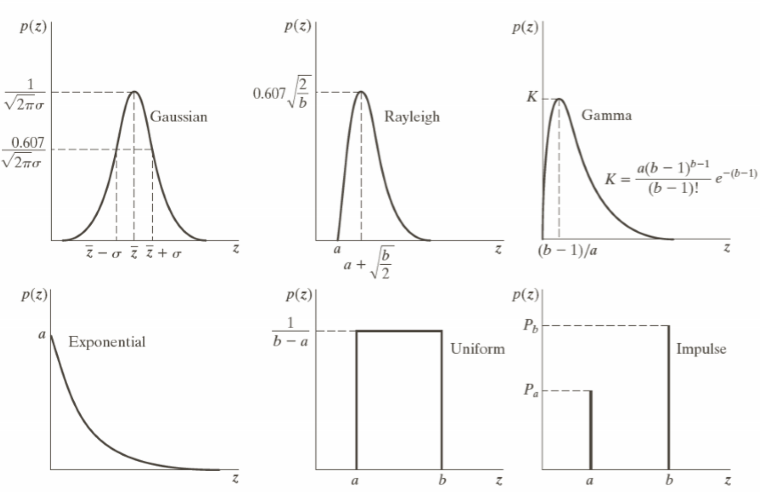
\includegraphics[width=\columnwidth]{Images/pdf_nois}
\end{center}

\subsubsection{Gaussian}
\[
p(z) = \frac{1}{\sqrt{2\pi}\sigma}e^{-\frac{(z-\overline{z}^2)}{2\sigma^2}}
\]

\subsubsection{Rayleigh}
\[
p(z) = \begin{cases}
	\frac{2}{b}(z-a)e^{-\frac{(z-a)^2}{b}} & for z \ge a \\
	0 & for z \lt a
\end{cases}
\]
Der Durchschnitt und Varianz können berechnet werden mit: 
\[
\overline{z} = a + \sqrt{\pi b / 4}
\]
\[
\sigma^2 = \frac{b(4-\pi)}{4}
\]

\subsubsection{Erlang (Gamma)}
\[
p(z) = \begin{cases}
	\frac{a^bz^{b-1}}{(b-1)!}e^{-az} & for z \ge 0 \\
	0 & for z \lt 0
\end{cases}
\]
Der Durchschnitt und Varianz können berechnet werden mit: 
\[
\overline{z} = \frac{a}{b}
\]
\[
\sigma^2 = \frac{b}{a^2}
\]

\subsubsection{Exponential}
\[
p(z) = \begin{cases}
	ae^{-az} & for z \ge 0 \\
	0 & for z \lt 0
\end{cases}
\]
Wobei $a,b \in \mathbf{N}^+$ sein muss. Der Durchschnitt und Varianz können berechnet werden mit: 
\[
\overline{z} = \frac{1}{b}
\]
\[
\sigma^2 = \frac{1}{a^2}
\]

\subsubsection{Uniform}
\[
p(z) = \begin{cases}
	\frac{1}{b-a} & for a \ge z \ge b \\
	0 & otherwise
\end{cases}
\]
Der Durchschnitt und Varianz können berechnet werden mit: 
\[
\overline{z} = \frac{a+b}{2}
\]
\[
\sigma^2 = \frac{(b-a)^2}{12}
\]

\subsubsection{Impulse (Salt-Pepper)}
Gut mit dem Hamonischen Mean Filter zu entfernen.
\[
p(z) = \begin{cases}
	P_a & for z = a \\
	P_b & for z = b \\
	0 & otherwise
\end{cases}
\]


\section{Reconstruction}
Grundsätzlich werden spatial Filter für das Wiederherstellen der Bilder benützt. Dabei ist ein Rechteck mit $m\times n$ und Zentrum $(x,y)$ als $S_{xy}$ definiert.

\textbf{Beispiel}
\begin{center}
	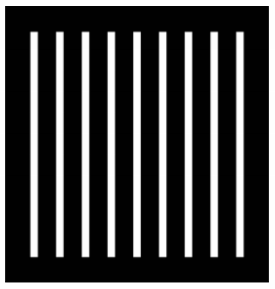
\includegraphics[width=0.2\columnwidth]{Images/iriginal}
\end{center}


\subsection{Arithmerisch}
\[
\hat{f} = \frac{1}{mn}\sum_{s,t\in S_{xy}}g(s,t)
\]
\begin{center}
	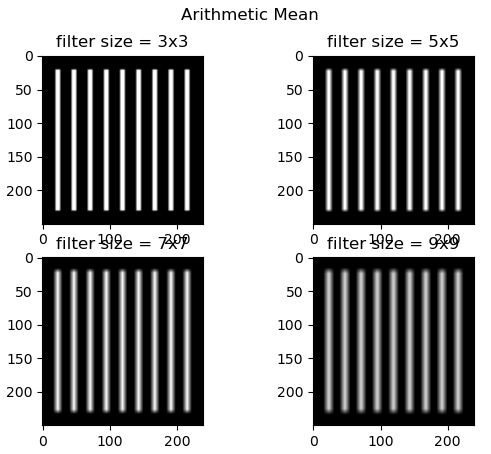
\includegraphics[width=0.8\columnwidth]{Images/ar}
\end{center}


\subsection{Geometric}
Smoothing ähnlich zu Arithmetrisch, aber weniger Details gehen verloren.
\[
\hat{f} = \left[\prod_{s,t\in S_{xy}}g(s,t)\right]^{\frac{1}{mn}}
\]

\subsection{Harmonic Mean}
\[
\hat{f} = \frac{mn}{\sum_{s,t\in S_{xy}}\frac{s}{g(s,t)}}
\]

Speziallfall ist dabei der Contraharmonie Mean Filter, welcher für positive $Q$ Pfeffer und negative $Q$ Salz Rauschen entfernt. Bei $Q=-1$ ist dies der Harmonic Mean Filter. $Q=0$ entspricht dem Arthmetrischen Mean Filter. Kann aber nicht gleichzeitig Pfeffer und Salz Rauschen entfernen.
\[
\hat{f} = \frac{\sum_{s,t\in S_{xy}}g(s,t)^{Q+1}}{\sum_{s,t\in S_{xy}}g(s,t)^Q}
\]
\begin{center}
	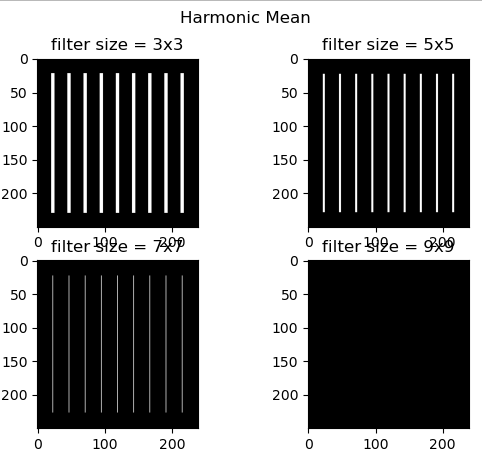
\includegraphics[width=0.8\columnwidth]{Images/harmonic}
\end{center}


\subsection{Order Statistic Filters}
Diese Filter basierend auf den Werten der Pixel.
\textbf{Median Filter} eignen sich gut für Impulse Noise.
\[
\hat{f} = \underset{(s,t)\in S_{xy}}\med g(s,t)
\]

\textbf{Max/Min}. Max reduziert also Pfeffer Rauschen, Min Salz Rauschen.
\[
\hat{f} = \underset{(s,t)\in S_{xy}}{\max/\min} g(s,t)
\]
\begin{center}
	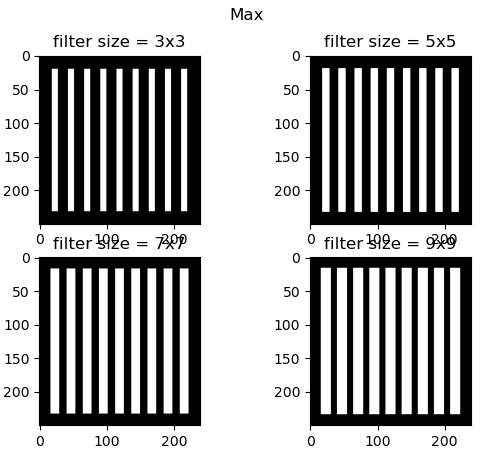
\includegraphics[width=0.8\columnwidth]{Images/max}
\end{center}


\textbf{Midpoint} funktioniert am besten bei zufällig verteiltem Rauschen, wie Gaußschem oder gleichmäßigem Rauschen.
\[
\hat{f} = \frac{1}{2}\left[\max g(s,t) + \min g(s,t)\right]
\]
\begin{center}
	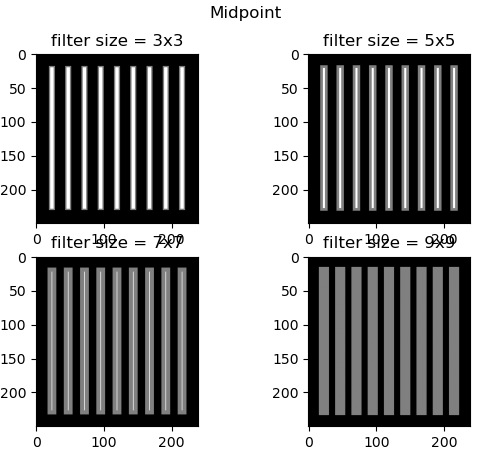
\includegraphics[width=0.8\columnwidth]{Images/max1}
\end{center}


\textbf{Alpha Trimmed}
Bestimmt den Mittelwert nur der mittleren $mn-d$ Werten. (Oft 80\%). Dieser Filter ist robust gegen Outliers und \textit{normales} Rauschen. Bei $d=0$ ist ein Aritherisches Filter. Bei $d = mn-1$ ist ein Median Filter.
\[
\hat{f} = \frac{1}{mn -d } \sum_{s,t\in S_{xy}}g(s,t)
\]